\documentclass[aspectratio=1610,compress,titleprogressbar]{beamer}
\usetheme{m}

\usepackage[british]{babel}
\usepackage{booktabs}
\usepackage{caption}
  \captionsetup[figure]{labelformat=empty}
  \captionsetup[table]{labelformat=empty}
\usepackage{fontspec}
\usepackage{fontawesome}
\usepackage[italic]{hepnicenames} \usepackage{microtype} \usepackage{minted}
  \usemintedstyle{trac}
\usepackage{multirow}
\usepackage{siunitx}
  \sisetup{separate-uncertainty=true}
\usepackage{unicode-math}

\title{Hlt2 Rate Monitoring in Run II}
%\subtitle{ZeroMQ All The Things!}
\author[K.~Dungs]{Roel~Aaij\inst{1} \and \textcolor{orange}{Kevin~Dungs\inst{2}}}
\institute{\inst{1} CERN \and \inst{2} TU Dortmund}

\begin{document}

\maketitle

\begin{frame}{Motivation}
  \begin{block}{Run II HLT}
    \begin{itemize}
      \item Split Hlt1 and Hlt2
      \item Events not processed in sequence any more (in Hlt2)
    \end{itemize}
  \end{block}
  \begin{block}{Why not DIM?}
    \begin{itemize}
      \item We had to write the infrastructure anyway
      \item Easier for us with ZeroMQ
      \item Also we \emph{wanted} to try it out :)
      \item DIM still used for steering
    \end{itemize}
  \end{block}
\end{frame}

\begin{frame}{ZeroMQ (ØMQ, ZMQ, \dots)}
  \begin{columns}
    \begin{column}{.6\textwidth}
      \begin{itemize}
        \item Message Queue
        \item Networking Library
        \item Concurrency Framework
        \item [] {}
        \item Developed by iMatix (P.~Hintjens)
        \item Written in C; Bindings for C++, Python, ...
        \item Open Source (LGPLv3)
        \item Widely used in industry (e.g. finance)
        \item [] {}
        \item \textbf{Crazy fast and scalable}
      \end{itemize}
    \end{column}
    \begin{column}{.4\textwidth}
      \begin{figure}
        \centering
        
\includegraphics[width=.8\textwidth]{graphics/zmq.png}
        \caption{\href{http://zeromq.org}{zeromq.org}}
      \end{figure}
    \end{column}
  \end{columns}
\end{frame}

\begin{frame}{Prototype}
  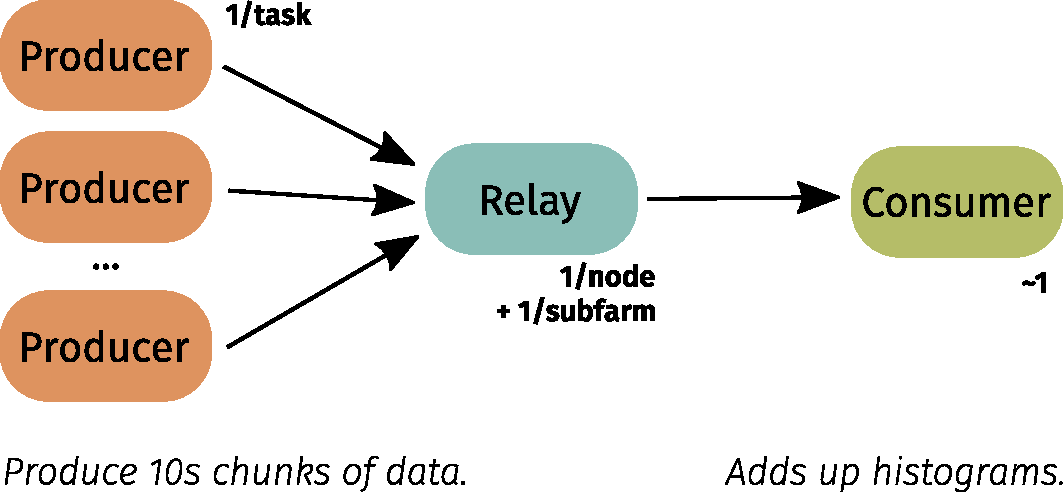
\includegraphics[width=\textwidth]{graphics/flow.pdf}
\end{frame}

\begin{frame}{Prototype}
  \begin{block}{Back of the Envelope Calculation}
    \begin{itemize}
      \item Use custom data structure for chunks of data \begin{itemize}
          \item TCK + identifier + relative time + array (\SI{10}{\second})
        \item Serialise with \texttt{boost::serialization}
      \end{itemize}
    \end{itemize}
    \begin{equation*}
      \SI{100}{Histograms} \times \SI{70}{\kilo Tasks} \times \SI{0.1}{\kilo B\per Event} \times \frac{\num{1}}{\SI{10}{\second}} = \SI{70}{\mega B\per\second}
    \end{equation*}

    \begin{itemize}
      \item \texttt{TFileBuffer} adds too much overhead (factor \numrange{8}{10})
    \end{itemize}
  \end{block}
\end{frame}

\begin{frame}{Testing on the Farm}
  \begin{itemize}
    \item ZeroMQ package for LHCb software
    \item Producer and Relay implemented as \texttt{Gaudi::Service}s
    \item Standalone consumer (for testing)
    \item [] {}
    \item One global consumer
    \item One relay per subfarm
    \item Per node: \begin{itemize}
      \item One relay
      \item $N$ producers ($N \approx 28 \dots 36$)
    \end{itemize}
  \end{itemize}
\end{frame}

\begin{frame}{What's next}
  \begin{itemize}
    \item Run on the full farm
    \item \textbf{Numbers!} (timing, throughput, ...)
    \item Interoperability with current (+new) presenter \begin{itemize}
      \item First: Histogram with 10 bins showing full rate of last processed run $-n$
      \item New presenter: Dynamic views!
    \end{itemize}
  \end{itemize}
\end{frame}

\end{document}
